\documentclass[9pt,twocolumn,twoside,lineno]{pnas-new}

%% Some pieces required from the pandoc template
\providecommand{\tightlist}{%
  \setlength{\itemsep}{0pt}\setlength{\parskip}{0pt}}

% Use the lineno option to display guide line numbers if required.
% Note that the use of elements such as single-column equations
% may affect the guide line number alignment.


\usepackage[T1]{fontenc}
\usepackage[utf8]{inputenc}

% Pandoc citation processing


\templatetype{pnasresearcharticle}  % Choose template

\title{Mobility and flexibility enable resilience of human harvesters to
environmental perturbation}

\author[a,1]{Owen R. Liu}
\author[b,c]{Mary Fisher}
\author[a]{Blake E. Feist}
\author[d]{Briana Abrahms}
\author[e]{Kate Richerson}
\author[a]{Jameal F. Samhouri}

  \affil[a]{Conservation Biology Division, Northwest Fisheries Science Center,
National Marine Fisheries Service, National Oceanographic and
Atmospheric Administration, 2725 Montlake Blvd E, Seattle, Washington
98112 USA}
  \affil[b]{School of Environmental and Forest Sciences, University of Washington,
Seattle, WA, 98195}
  \affil[c]{NSF Graduate Research Internship Program, Northwest Fisheries Science
Center, National Marine Fisheries Service, National Oceanographic and
Atmospheric Administration, 2725 Montlake Blvd E, Seattle, Washington
98112 USA}
  \affil[d]{Center for Ecosystem Sentinels, Department of Biology, University of
Washington, Seattle, WA 98195}
  \affil[e]{Fishery Resource Analysis and Monitoring Division, Northwest Fisheries
Science Center, National Marine Fisheries Service, National
Oceanographic and Atmospheric Administration, Newport, OR, 97365}


% Please give the surname of the lead author for the running footer
\leadauthor{Liu}

% Please add here a significance statement to explain the relevance of your work
\significancestatement{Large-scale environmental perturbations like heatwaves will likely
become more common under climate change. Sustainability in
social-ecological systems requires an understanding of behaviors that
can promote resilience to these perturbations. We show how participants
in a valuable fishery used spatial mobility and fishing portfolio
diversification to buffer against negative effects of a record marine
heatwave. Our data-driven approach combines satellite movement data with
economic data to reveal adaptive behaviors, and can be used to inform
the study of human harvesters dynamics in other social-ecological
systems.}


\authorcontributions{O.R.L., M.F., B.E.F., B.A., K.R., and J.F.S. designed research; O.R.L.
and J.F.S. performed research and analyzed data; O.R.L., M.F., B.E.F.,
B.A., K.R., and J.F.S. wrote the paper.}

\authordeclaration{The authors declare no conflict of interest.}


\correspondingauthor{\textsuperscript{} }

% Keywords are not mandatory, but authors are strongly encouraged to provide them. If provided, please include two to five keywords, separated by the pipe symbol, e.g:
 \keywords{  climate change adaptation |  environmental perturbation |  marine heatwave |  fisheries dynamics  } 

\begin{abstract}
Characteristics of natural resources that enable sustainable management
are often more fully understood than the adaptive behaviors of human
harvesters in those same systems. Given increasing environmental
variability due to climate change, it is especially critical to
understand how human harvesters may respond to environmental
perturbation. In this study, we identify characteristics that promoted
resilience of one the most valuable fisheries on the west coast of the
United States to a record marine heatwave. Using movement telemetry
linked to fishery landings records from more than 500 fishing vessels,
we found that vessels employed two, non-mutually exclusive strategies to
cope with the anomalous environmental and management conditions imposed
by the heatwave: increasing spatial mobility and diversifying fishery
participation. The combination of these strategies appeared to be
adaptive, as it produced the greatest increase in profits. Our
data-driven approach reveals behaviors that can be promoted to increase
harvest sustainability and can inform management in other
social-ecological systems in which human harvester dynamics are poorly
understood.
\end{abstract}

\dates{This manuscript was compiled on \today}
\doi{\url{www.pnas.org/cgi/doi/10.1073/pnas.XXXXXXXXXX}}

\begin{document}

% Optional adjustment to line up main text (after abstract) of first page with line numbers, when using both lineno and twocolumn options.
% You should only change this length when you've finalised the article contents.
\verticaladjustment{-2pt}

\maketitle
\thispagestyle{firststyle}
\ifthenelse{\boolean{shortarticle}}{\ifthenelse{\boolean{singlecolumn}}{\abscontentformatted}{\abscontent}}{}

% If your first paragraph (i.e. with the \dropcap) contains a list environment (quote, quotation, theorem, definition, enumerate, itemize...), the line after the list may have some extra indentation. If this is the case, add \parshape=0 to the end of the list environment.

\acknow{M. Fisher was supported in part by the NSF's Graduate Research
Fellowship Program (Grant DGE-1762114)}

Sustainability in social-ecological systems---the continued provision of
human and ecological benefits from healthy ecosystems (1)---requires
resilience to environmental perturbations. Often, though, people respond
to environmental change in diverse and complex ways. Just as multiple
species occupying similar ecological niches may react differently to
physical changes in their environments (2), human actors in a
social-ecological system can exhibit diverse behaviors within the
constraints imposed by the governance system (3). Groups of resource
users with distinct livelihood portfolios, available capital, or spatial
patterns of resource extraction will not respond the same way to
environmental or management changes(4). In response to change, some
users might stick to established knowledge and reliable spatial patterns
of exploitation, while others might employ more exploratory strategies
that carry higher potential upsides but also higher risks and costs.
Understanding the adaptive behaviors of resource users is all the more
important given the increasing prevalence of extreme climate events
attributable to climate change (5--8), but empirical evidence making the
link between climate extremes and contemporaneous human adaptation
remains lacking.

Fisheries are a prominent example of a social-ecological system where
complex links between resource user (harvester)behavior and natural
resource dynamics drive sustainability(9). Fisheries represent the last
large-scale wild harvest of food on Earth, but also one of the most
traditional livelihoods in human history. Difficulties in achieving
sustainability in fisheries have often been linked to an inadequate
understanding of harvester dynamics(10, 11). Differences in fisher
behaviors, both within and across fisheries, can affect the stability
and sustainability of fish populations(12, 13) and of other
species---for instance, endangered marine mammals or seabirds(14, 15).

Additionally, different behavioral segments of fishing fleets may
respond in different ways to management measures, or may be
differentially vulnerable to environmental perturbations (12). For
example, (16) found that more exploratory fishing vessels---those that,
on average, traveled further and more often traversed new fishing
grounds---were better able to cope with an extended spatial closure.
These fisher responses, however, are difficult to study, despite the
potential impact of differential behavioral responses on resource
dynamics. Partly, this is due to a lack of detailed spatial and economic
information on harvester behavior. However, recent years have seen a
rise in availability of these types of fishery data, paired with methods
to extract behavioral insights from them (17--19). In the following, we
apply a range of data-driven methods to ask: how did human harvesters
cope with and adapt to a major environmental perturbation in the most
valuable fishery on the U.S. west coast?

The Dungeness crab fishery on the west coast of the United States often
obtains in excess of \$200 million in revenue from over 1,000
participating vessels each year(20, 21). It is a fishery that is central
both ecologically (22) and economically (23) to the west coast
social-ecological system, making it at once a safety valve within
fishers' portfolios and a source of complexity in fisheries
governance(24, 25). The Dungeness crab fishery appears able to withstand
immense fishing pressure, and although crab abundance can fluctuate
markedly from year to year, long term abundance has been relatively
stable for more than a half century (21).

\begin{figure}%[tbhp]
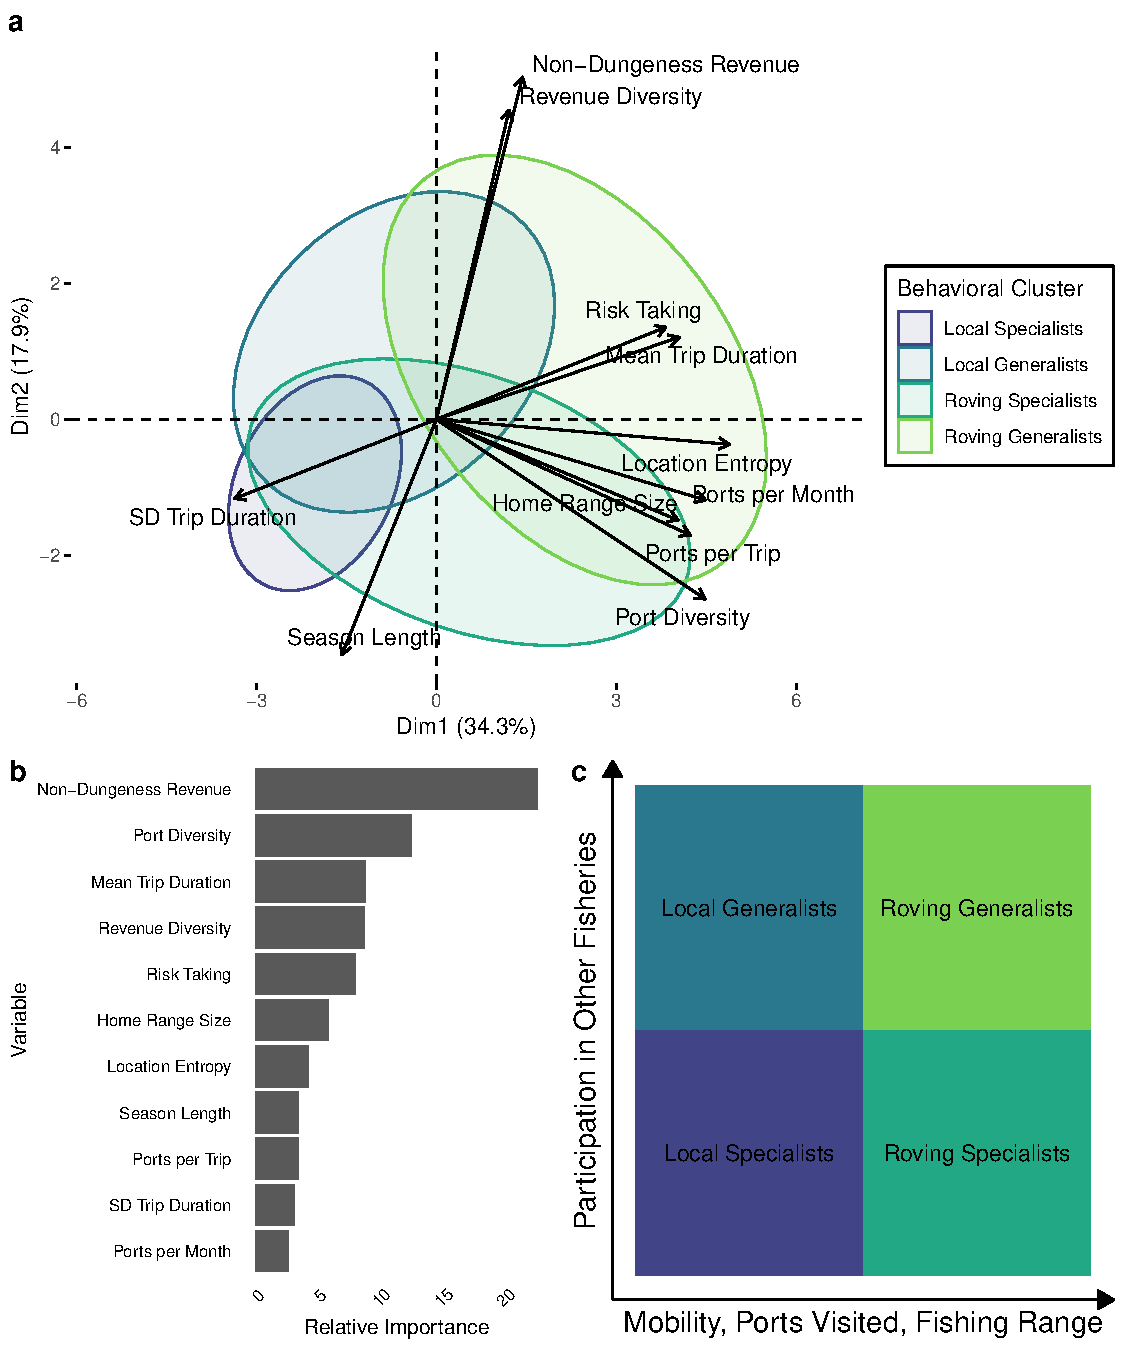
\includegraphics[width=\linewidth]{fig_pca_rf.pdf}
\caption{Data-driven formation of fishing behavioral groups. (a) Principal component analysis of vessel-seasons. Clusters of vessel-seasons, which determine behavioral groups, are enclosed by ellipses. Arrows represent the association between metrics in the cluster analysis relative to the placement of vessel-seasons. (b) Ranked importance of top variables used to classify vessel-seasons into behavioral groups, as determined by random forest analysis.(c) Conceptual visualization of the major axes defining behavioral groups.}
\label{fig:pca}
\end{figure}

However, recent environmental shocks have challenged the social
sustainability of the Dungeness crab fishery. In 2014-2016, a record
marine heatwave (MHW) led to a harmful algal bloom of unprecedented
scale(26), causing toxin levels in Dungeness crabs to reach levels
dangerous for human consumption and correspondingly lengthy delays in
large regions of the coast in the 2015-16 and 2016-17 Dungeness fishing
seasons. Concurrently, the MHW caused shoreward compression of the
preferred feeding habitat of large whales, contributing to a rise in
entanglements of whales in Dungeness crab fishing gear and increasing
risk of fishery closure due to marine mammal interactions, effects that
continued to directly affect fishery closures through the 2017-18
Dungeness crab season (22, 27). During this period, Dungeness crab
fishers had to contend with significant ecological changes and with the
management measures those changes precipitated. Like with climate
extremes in other systems(28), the effects of this MHW were complex,
reverberated through the social-ecological system, and persisted for
years after the anomalous warming dissipated(29, 30). While much recent
literature is dedicated to examination of biophysical and ecological
impacts of the MHW (26, 32), to date far less attention has been given
to exploring how social systems cope and change with these
perturbations(33).

In this study, we compare the adaptive responses of behavioral groups
within the Dungeness crab fishery to the multi-year MHW that directly
affected the 2015-16 through 2017-18 Dungeness crab seasons. The 2015-16
Dungeness crab season was the first season to be significantly delayed
as a direct result of ecosystem changes, a trend that continued through
the 2017-18 season. While previous work has investigated economic
impacts(25, 33) and changes in fishery participation due to the
MHW-associated harmful algal bloom(31), here we explicitly investigate
and quantify fishers' adaptive spatial behaviors in response to the MHW
more broadly and for the full three-year period over which the MHW
impacts manifested. Using a 10-year time-series of more than 2 million
satellite-derived fishing vessel location records, linked to fishery
revenue and landings data, we derive quantitative behavioral metrics
describing space use and mobility of Dungeness crab vessels, then
organize these behaviors into characteristic behavioral groups. We
explore the overlap of spatial behaviors with profitability, fishing
season length, and revenue diversity. We track these behavioral groups
over time, and identify key behavioral metrics that promoted adaptation
during and after the MHW. This analysis therefore offers insights into
the types of adaptive behaviors that may promote sustainable outcomes
for human harvesters in social-ecological systems more broadly.

\hypertarget{results}{%
\subsection*{Results}\label{results}}
\addcontentsline{toc}{subsection}{Results}

\hypertarget{describing-fisher-behavior}{%
\subsubsection*{Describing Fisher
Behavior}\label{describing-fisher-behavior}}
\addcontentsline{toc}{subsubsection}{Describing Fisher Behavior}

We characterized fisher behavior using variables derived from vessel
telemetry and fisheries landings data. The combined dataset based on 596
different vessels spanned 11 fishing seasons (2008-2019), with
\textasciitilde2.2 million satellite-derived Vessel Monitoring System
(VMS) geolocations, and 315,000 fishery landing records. Using these
combined data, we analyzed 11 behavioral variables in five general
behavioral categories: fishing port use, fishing trip characteristics,
participation in other fisheries, risk-taking behavior, and exploration
and mobility (definitions of all metrics are provided in Table S1). Our
choice of behavioral variables to calculate was driven by previous
evidence of the importance of each variable in describing fisher
behavioral patterns(16, 23, 34, 35). Each of the fisher behavioral
variables described one characteristic of a vessel's apparent behavior
over the course of a fishing season---a vessel-season.

Using a hierarchical clustering algorithm (see Methods), we found that
the 3391 vessel-seasons in our data fell into four behavioral cluster
groups (Fig. \ref{fig:pca}a). The most important discriminating
variables driving the clustering were proportion of revenue from
non-Dungeness crab fisheries, followed by diversity of port use, revenue
diversity, and mean trip duration (Fig. \ref{fig:pca}b). These analyses
suggest that the behavior of the four groups can be conceptualized as
varying along two major axes (Fig. \ref{fig:pca}c)--- (1) spatial
mobility (principal component 1 in Fig. \ref{fig:pca}a) and (2)
propensity to fish in non-Dungeness crab fisheries (fishery flexibility,
principal component 2 in Fig. \ref{fig:pca}a).

Vessels with higher spatial mobility, which we term Roving groups, move
between ports throughout a fishing season and have large fishing ranges,
while those with lower mobility--- Local groups---show greater fidelity
to a single port. Vessels with greater fishery flexibility, deemed
Generalist groups, have high revenue diversity and derive a relatively
greater portion of their total fishery revenue from fisheries other than
Dungeness crab. Vessels exhibiting less
flexibility---Specialists---concentrate fishing effort within the
Dungeness crab fishery. A vessel-season is therefore defined as either
Roving or Local, and either Specialist or Generalist. As an example, for
crab vessels fishing out of Newport, Oregon, Local Specialists have the
smallest fishing grounds, followed by Local Generalists, Roving
Specialists, and Roving Generalists (Fig \ref{fig:characteristics}a).
Across all vessel-seasons, Generalist vessels have shorter crab fishing
seasons, exiting the Dungeness crab fishery earlier to pursue other
fishing opportunities, while Specialists continue to garner a large
percentage of their weekly landed revenue from Dungeness crab over the
course of the season (Fig. \ref{fig:characteristics}b).

\begin{figure}%[tbhp]
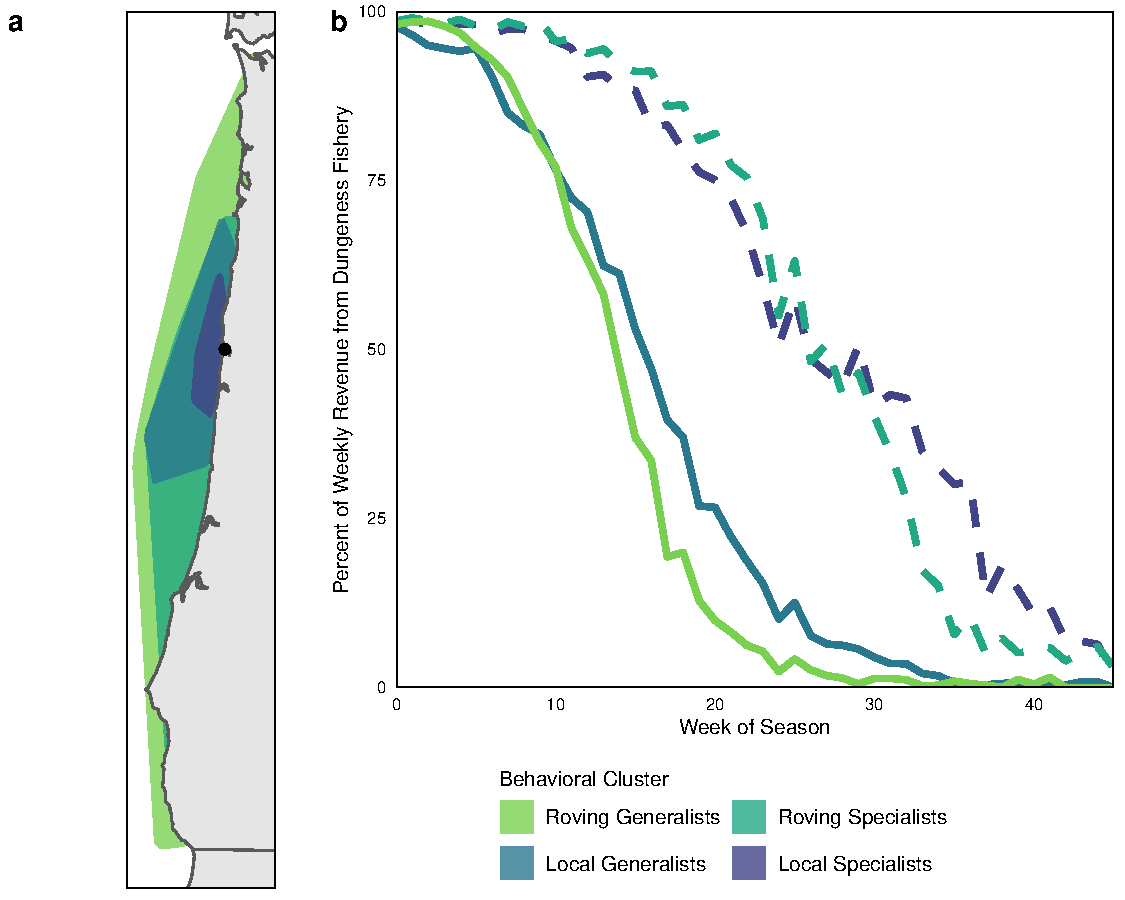
\includegraphics[width=\linewidth]{groups_mobility_flexibility.pdf}
\caption{Characteristic patterns in spatial mobility and fishery flexibility across behavioral groups in the west coast Dungeness crab fishery, exemplified by an Oregon port. (a) Fishing footprints of each behavioral group across all seasons for vessels originating from the Port of Newport, Oregon, USA. Shaded polygons are 95 percent convex hulls of all VMS locations for each group. (b) Fishery flexibility, displayed as the mean percent of total weekly revenue obtained from the Dungeness crab fishery (relative to all other fisheries) by vessels in each behavioral group. Weekly revenues are averaged across crab seasons and across all vessels in each group. Generalist groups are represented with solid lines, while Specialist groups are represented with dashed lines.}
\label{fig:characteristics}
\end{figure}

\hypertarget{behavioral-changes-during-the-marine-heatwave}{%
\subsubsection*{Behavioral Changes During the Marine
Heatwave}\label{behavioral-changes-during-the-marine-heatwave}}
\addcontentsline{toc}{subsubsection}{Behavioral Changes During the
Marine Heatwave}

The four fishing behavioral groups defined by our cluster analysis
responded to the social-ecological disruption of the marine heatwave
(MHW) by increasing their dependence on other, non-Dungeness fisheries
and expanding their fishing ranges. All groups had higher non-Dungeness
fishery revenue during the MHW period than during other seasons,
indicating a potential fallback to other fisheries during a period of
delays and management disruptions in the crab fishery (Fig.
\ref{fig:revenue})(31, 37). The 2016-17 and 2017-18 seasons had the
highest non-Dungeness crab revenue in the time series (Fig.
\ref{fig:revenue}a). The Generalist groups in particular more than
doubled their revenues from non-Dungeness fisheries (ANOVA p \textless{}
0.01; Fig. \ref{fig:revenue}b). The Specialist groups also had greater
non-Dungeness revenues during the MHW period, but the differences were
not as substantial as for the Generalist groups (Table S2, ANOVA p =
0.06 for Roving Specialists, p=0.99 for Local Specialists).

Some Dungeness fishers also expanded their Dungeness crab fishing
grounds during the MHW, particularly the two Roving groups (Fig.
\ref{fig:homerange}). Prior to the MHW (2008-15), Roving Generalists had
the largest mean home range size at more than 4000 square kilometers
(Fig. \ref{fig:homerange}a). Roving Specialists had the second-largest
ranges on average (around 2500 square kilometers), while the Local
groups had much smaller ranges (less than 1000 square kilometers). In
the MHW period from 2015-18, the Roving groups fished significantly
larger areas, with the Roving Generalist and Roving Specialist groups
averaging more than 5500 and 3500 square kilometers fished, respectively
(p=0.001 and p\textless\textless0.001 for Roving Specialists and Roving
Generalists). In contrast, the areas fished for the Local groups did not
change significantly (Fig. \ref{fig:homerange}b and Table S3 ,
p\textgreater0.99 for both Local groups). For all four groups, within
the MHW period, the most pronounced change in mobility occurred during
the 2016-17 fishing season.

\begin{figure}%[tbhp]
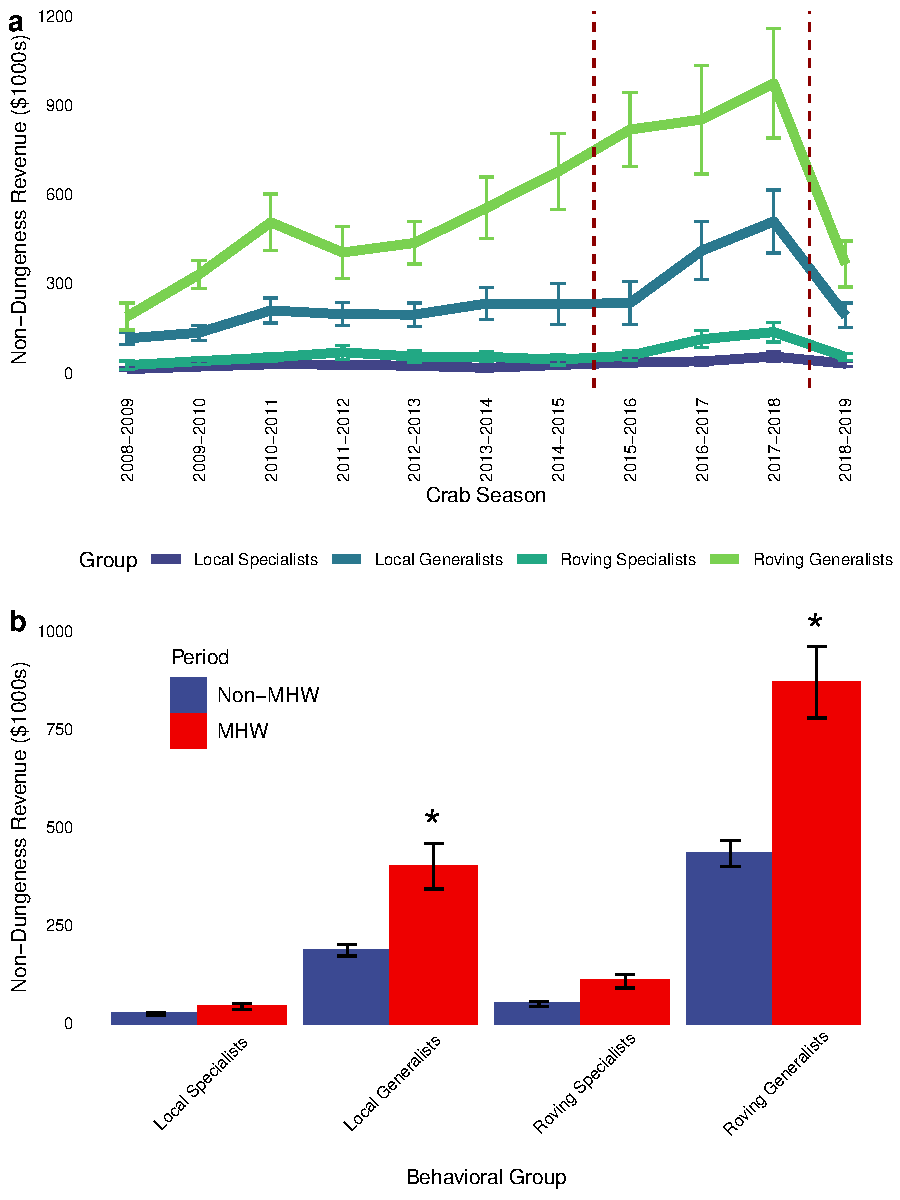
\includegraphics[width=\linewidth]{fig_nondcrb_revenue.pdf}
\caption{Non-Dungeness revenue for vessels in the analysis. (a) Seasonal mean revenue (+/- 2SE) for vessels in each behavioral group coming from all non-Dungeness fisheries combined. Vertical lines delineate the period of the marine heatwave (MHW). (b) Barplot of mean revenue (+/- 2SE) for vessels in each group during MHW and non-MHW seasons. Stars indicate groups with significantly different non-Dungeness revenue in MHW seasons.}
\label{fig:revenue}
\end{figure}

\hypertarget{profitability-of-behavioral-groups-during-the-marine-heatwave}{%
\subsubsection*{Profitability of Behavioral Groups during the Marine
Heatwave}\label{profitability-of-behavioral-groups-during-the-marine-heatwave}}
\addcontentsline{toc}{subsubsection}{Profitability of Behavioral Groups
during the Marine Heatwave}

An open question is whether the adaptive responses we detected and
quantified-- greater spatial mobility and more flexible fishing--
allowed fishers to maintain profits in the face of this major
environmental perturbation. To address this question, we modeled costs
of fishing for Dungeness crab based on vessel size and trip length (see
Methods). Our fishing cost model provides an estimation of Dungeness
crab profit (reported revenue minus estimated cost) for every fishing
trip in the data (i.e., for those vessels that continued to fish), and
allowed us to describe how profits within each behavioral group varied
over time (Fig. \ref{fig:profits}).

For all groups, average revenues and estimated costs both increased
during the MHW period, but revenue increases outweighed the increases in
cost, resulting in increased profits. Dungeness crab profits for all
behavioral groups increased during the MHW, significantly so for Local
Generalists (p=0.05), Roving Generalists (p\textless\textless.0001) and
Roving Specialists (p=0.001, Table S4). The Roving Generalist group saw
the largest increase in estimated profits in both raw and percent
increase in profits (more than a \$63,000 increase per vessel, a 48
percent increase, on average). Local Specialists experienced the
smallest increase in profits of all groups (25 percent) during the MHW,
while Roving Specialists and Local Generalists experienced a greater
than 40 percent increase. In the season after the dissipation of the
MHW, estimated profits declined, particularly for the Roving groups.

\begin{figure}%[tbhp]
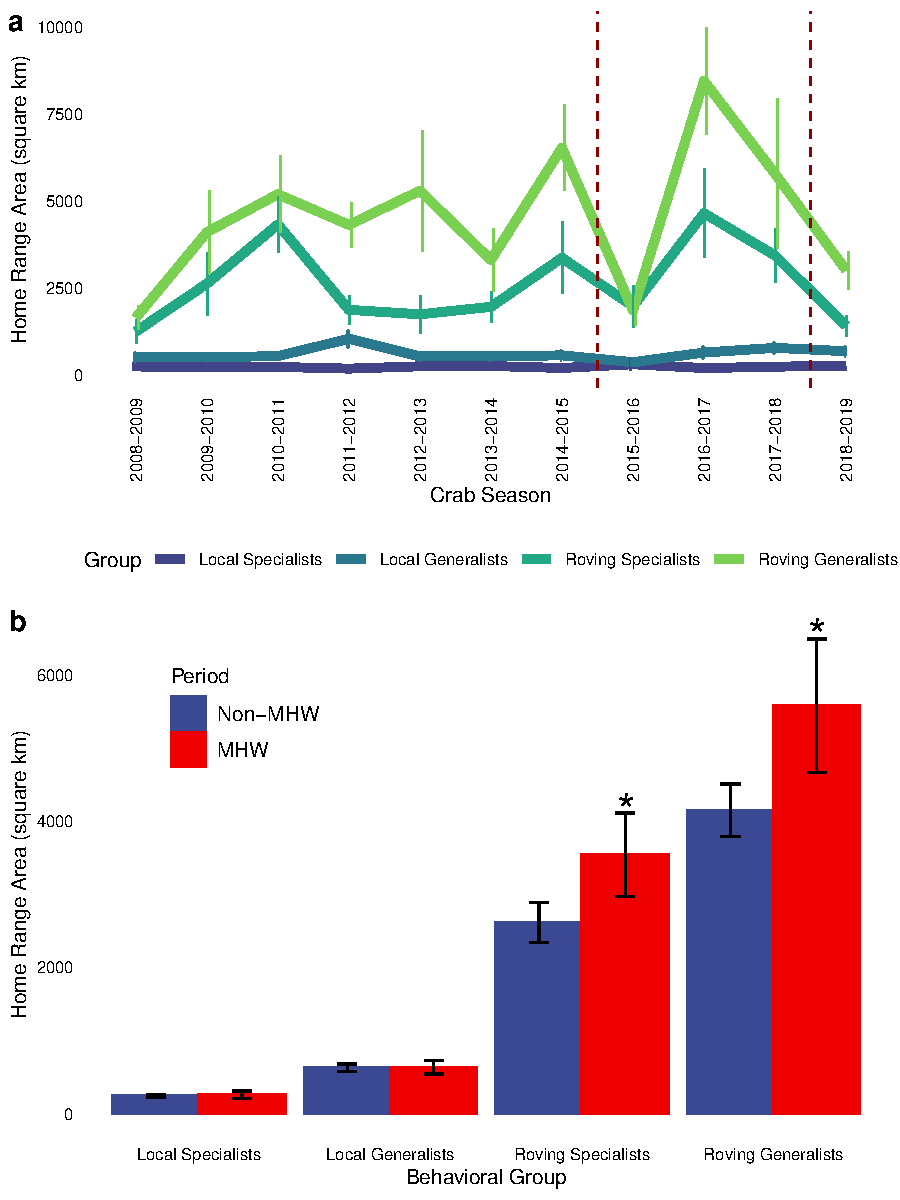
\includegraphics[width=\linewidth]{fig_homerange.pdf}
\caption{Home range (fishing area) size for vessels in the analysis. (a) Seasonal mean home range area in square kilometers (+/- 2SE) for vessels in each behavioral group. Vertical lines delineate the period of the MHW. (b) Barplot of mean home range area (+/- 2SE) for vessels in each group during MHW and non-MHW seasons. Stars indicate groups with significantly different home range size during MHW seasons.}
\label{fig:homerange}
\end{figure}

\hypertarget{discussion}{%
\subsection*{Discussion}\label{discussion}}
\addcontentsline{toc}{subsection}{Discussion}

The pace and magnitude of environmental change demand assessment of how
social-ecological systems will respond. Ideally, management approaches
can be designed to help humanity adapt by meeting the basic needs of
people without compromising ecosystems for future generations (38). As
one of the last remaining hunter--gatherer activities occurring at
scale, commercial fisheries offer an important lens through which to
understand human adaptations to novel and extreme conditions, with
potential lessons for other natural resource harvesting contexts. The
2014-2016 MHW on the U.S. west coast stressed the adaptive ability of
participants in the highly lucrative Dungeness crab fishery, because an
environmental perturbation (the MHW and associated harmful algal bloom
and shoreward compression of large whale habitat) led to cascading
regulatory actions and market effects (37). Our analysis revealed that
Dungeness crab fishers that remained in the fishery responded to
unprecedented environmental and management changes in multiple ways.
Behavioral groups characterized by spatial mobility used expanded
fishing grounds in the 2016-17 and 2017-18 seasons to maintain or
increase revenues. Similarly, fishers with strategies based around
diversified fishing portfolios---Generalists---were able to increase
their revenue from other fisheries to bolster their total fishing
income. We found that vessels combining greater spatial mobility with
higher participation rates in other fisheries were the most profitable,
and that these financial benefits were maintained or magnified during
the MHW. The behavioral strategies observed in the Dungeness crab
fishery may suggest pathways to improve adaptive capacity for human
harvesters more broadly during an era in which the magnitude, frequency,
and intensity of environmental perturbations are increasing.

The relative ability of specialists and generalists to cope with
environmental change has been investigated in the economics (39),
evolution (40), and ecology (41) literatures. The cross-disciplinary
consensus is that generalists may adapt better to increasingly variable
environments. Smith and McKelvey (1986)(39) suggested that specialists
and generalists in fisheries use different strategies to cope with
variability and uncertainty in income---specialists are efficient and
minimize income risk through fishery-specific acumen, while generalists
hedge against risk by building diverse portfolios(42). In a direct
ecological analogy, generalist consumers in an ecosystem experiencing
novel environmental conditions may be able to gain a competitive
advantage over specialists by efficiently switching to alternative prey
sources(41). While management dynamics, markets, stochastic resource
abundance, and conditions in other fisheries are complicating factors
(37), the relative performance of specialist versus generalist
strategies in the Dungeness crab fishery largely adhere to these
existing economic and ecological models. Although some Specialists and
Generalists persisted through the MHW period, repeated environmental
disruptions in the future that cause further seasonal and spatial
restrictions on the Dungeness crab fishery may begin to favor a
Generalist strategy. Within the US west coast context, existing fishery
governance systems may constrain this type of generalist adaptation
(43), but there are calls for ``climate-ready'' fisheries that include
the flexibility for fishers to move between fisheries (44). A better
understanding of the social, economic, and cultural drivers of fishers'
decisions to be specialists or generalists is a core component of a
sustainable livelihoods approach to small-scale fisheries management
(45). Such an approach can also offer insights for the design of
regulatory approaches that facilitate resilience to environmental
perturbation in larger-scale fisheries and natural resource management
contexts (12).

Diversification of fishery revenue was not the only axis of variation
associated with persistence in the face of the MHW. Spatial mobility was
also a key component of the fishing strategies we observed. Following
others who have used recently emerging technologies to understand the
sustainability of human harvester strategies (46--48), we used satellite
data to characterize the spatial behavior of vessels. Roving groups,
whether Specialists or Generalists, were more profitable than their
Local counterparts under all conditions. The benefits of this spatial
mobility were clear during the marine heatwave. We hypothesize that
roving vessels were the most capable of responding to management
actions, market forces, and ecological factors (e.g., product quantity
and quality) that shifted spatially during the heatwave. The ability of
more exploratory fishers to cope during an environmental disturbance has
recently been demonstrated in other systems(16), and our findings
confirm that more mobile vessels performed better during the
environmental perturbation. Similar patterns have been shown among
foraging marine mammals, where individual animals that are more
exploratory have greater foraging success during anomalous climate
conditions than more site-faithful conspecifics (49).

\begin{figure}%[tbhp]
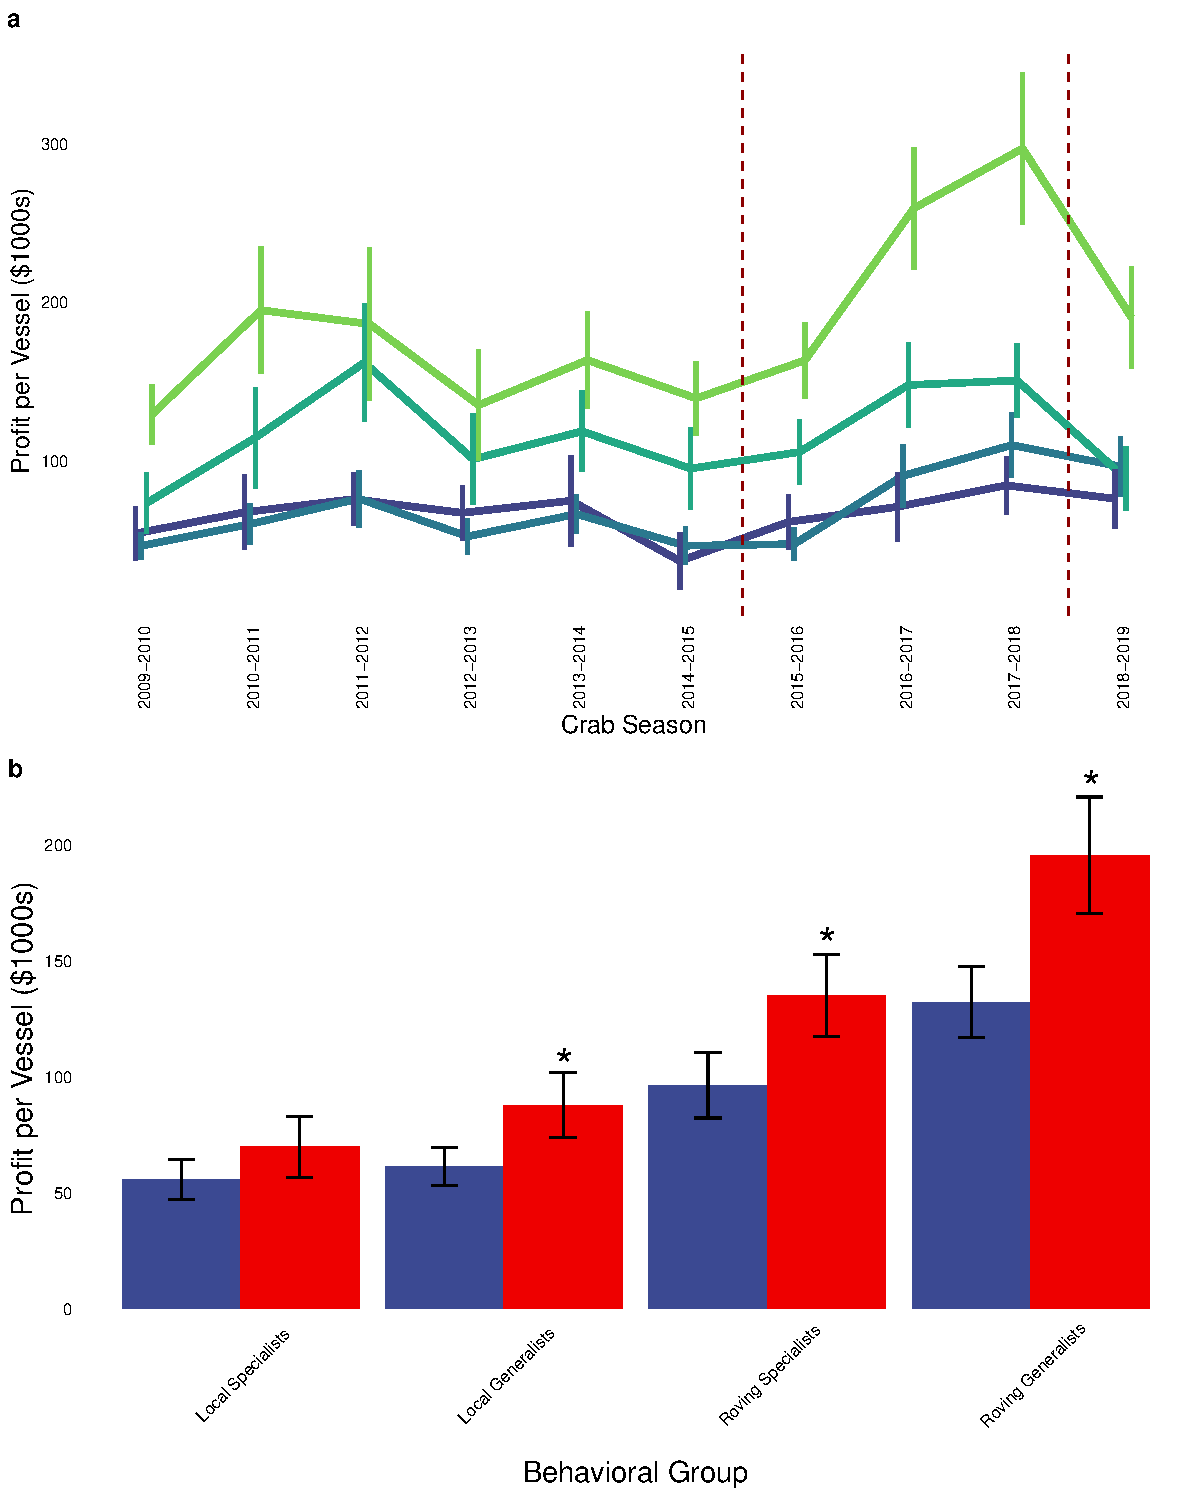
\includegraphics[width=\linewidth]{fig_profits.pdf}
\caption{Estimated profits by behavioral group. (a) Mean profit (+/- 2 SE) for vessels in each behavioral group over the full crab season. Vertical lines delineate the period of the marine heatwave. (b) Mean profit (+/- 2 SE) for each group in heatwave (MHW) versus non-MHW seasons. Stars indicate groups with significantly different estimated profits during MHW seasons.}
\label{fig:profits}
\end{figure}

Importantly, the nature of the data used in this study means that we
studied the behavior of the `survivors'---that is, the fishers who
decided or were able to remain in the Dungeness crab fishery during the
MHW period. The MHW acted as a selective force on Dungeness crab fishery
participation. Many Dungeness crab fishers during the 2016 and 2017
fishery closures chose (or were forced by circumstance) to not
participate in the fishery at all, instead opting to exit fishing
entirely or to re-concentrate all effort in alternative fisheries (31).
Some of the relative success of the Dungeness crab fishers during the
MHW observed in this study, therefore, may be due to reduced
competition, as well as periods of supply shortages and high prices.
Although outside the scope of the current analysis, an important area
for further research is to determine how and why, when faced with an
environmental perturbation, fishers choose to remain or exit a fishery
(50).

With climate change expected to increase the frequency of extreme
environmental perturbations like MHWs (6), established patterns of
natural resource management and human harvester behavior will be
challenged. In our study, following multiple adaptive pathways by both
diversifying and mobilizing appears to be one solution to an extreme
environmental event and rapid management changes in the Dungeness crab
fishery. Management measures that restrict the fishery temporally or
spatially---such as spatially-explicit biotoxin-related closures or
early termination of the fishing season due to risk of interactions with
protected or bycatch species---will differentially affect distinct
groups of fishers. Single-fishery specialists may thrive when the
harvested resource is stable and productive, but these fishers may
struggle to adapt if management measures restrict fishing season
lengths. Likewise, localized fishers can thrive through intimate
knowledge of fishing grounds, but if large-scale environmental
perturbations have spatially-explicit negative effects, fishers with
knowledge of a wider array of fishing grounds and greater mobility will
naturally gain an advantage (16). Over time, management context, or
failures of management to adapt, can drive changes in the makeup of
fishing fleets as a whole (47). These changes are not inherently
negative, but in order to maintain the social, economic, and cultural
benefits provided by a fishery, managers should endeavour to anticipate
behavioral changes within fleets. More generally, these insights are
congruent with an evolving understanding of adaptation in complex
social-ecological systems (38). Because complex systems are an emergent
product of the individual actions of human actors, informed adaptive
management requires an understanding of the drivers of behaviors like
those identified in this study along with well-calibrated and nimble
responses within governance systems.

For fishers and other human harvesters, future work using mixed methods
from the social sciences like participatory mapping and semi-structured
interviews (50, 51) will provide complementary insights into the
motivations and social drivers behind adaptive decisions. Furthermore,
as integrated biophysical and socioeconomic data streams become
increasingly available for environmental management (53), data-driven,
interdisciplinary studies of resilience and adaptation will enable
dynamic management of natural resources (54, 55). This push for the
incorporation of multiple data streams in environmental management
extends beyond marine fisheries---for example, in wildland fire
management in the United States, integrated data platforms that combine
geospatial data with risk models and fuel treatment scenarios are
leading to a more predictive and adaptable landscape and fire management
plans (56, 57).

This study revealed the elements of behavioral diversity among human
harvesters in a lucrative keystone fishery, and described how those
elements enabled adaptation during an extreme environmental event
attributable to climate change (58). Just as biological response
diversity can lead to enhanced ecosystem resilience to environmental
change (2), behavioral diversity among natural resource users may
promote resilience of social-ecological systems. Given the impending
increase in extreme climatic events such as marine heatwaves (29, 59),
recognition of social and ecological traits that enable resilience now
can help to build toward a more prepared future. Behavioral analyses
like ours can be used in the design of adaptive management measures, to
bolster policy analyses, and to inform decision-making under
environmental uncertainty.

\hypertarget{methods}{%
\subsection*{Materials and Methods}\label{methods}}
\addcontentsline{toc}{subsection}{Materials and Methods}

\hypertarget{data-sources}{%
\subsubsection*{Data sources}\label{data-sources}}
\addcontentsline{toc}{subsubsection}{Data sources}

We used satellite-based Vessel Monitoring System (VMS) data and port
level fishery landings data to define most of the behavioral variables.
The VMS database is maintained by the National Marine Fisheries
Service's Office of Law Enforcement, and records the positions of
vessels at approximately one hour intervals. Similar VMS data has been
used in other studies of fishery spatial dynamics (17, 18, 27, 34). A
subset of the vessels that participate in the Dungeness crab fishery are
equipped with VMS transponders (primarily vessels that also participate
in the west coast groundfish fishery, where VMS transponders are
mandatory). This subset varies between 19 and 26 percent of all vessels
recording landings for Dungeness crab between the 2008-2009 and
2018-2019 seasons, representing between 10 and 57 percent of all
Dungeness crab landings by weight, and between 15 and 42 percent of
Dungeness revenue, depending on the year and state (California, Oregon,
or Washington). Oregon has the highest relative VMS representation,
followed by California, then Washington.

Fish ticket information was obtained through the Pacific Fisheries
Information Network (PacFIN). These data represent 1949 vessels
targeting Dungeness crab in California, across more than 300,000 fish
tickets (i.e., fishing trips). Fishing trips were defined as targeting
Dungeness crab if the total landings of Dungeness on the individual fish
ticket were at least 10 percent greater than the landed weight of the
next greatest species.

We joined the fish ticket data to the VMS data through unique vessel
identification numbers and timestamps. VMS geolocations comprising a
fishing trip were defined as all of the geolocations between a landed
fish ticket and the one immediately preceding it (i.e., the previous
ticket landed by the same vessel). After joining the VMS and fish ticket
data, we removed trips in which the final VMS data point for a trip was
greater than 50km from the port of landing recorded on the ticket.
Finally, we removed VMS records from vessels sitting idle in port. To do
so, we truncated all but the first and last VMS records for each trip
that fell within a small buffer zone (1.5 to 3 km) around each port of
landing and with an average calculated speed of less than 0.75 m/s.

Dungeness crab fishing seasons on the west coast typically begin in the
middle of November (for Central California) or beginning of December
(for Northern California, Oregon, and Washington), but can be variable
in their starting dates, depending on state (California, Oregon, or
Washington), harmful algal bloom closures, price and market conditions,
crab condition and meat quality, and potential interactions with
protected species like humpback whales. Therefore, we used a data-driven
approach to define the start date for each crab season in each of the 20
fishing port groups on the west coast. Port groups are defined by PacFIN
and include clusters of small, neighboring fishing ports. For each port
group in each season, we found the date after October 31 of each season
that the total Dungeness crab landings into that port reached 1 percent
of the eventual, season-long landings. This approach identifies the
realized start date of the crab fishery in each portion of the coast in
each year.

The maximum length of a Dungeness fishing trip was defined as seven days
(S. Jardine, pers. comm.). That is, if there was a gap of greater than
seven days between consecutive tickets, the VMS geolocations greater
than seven days prior to the landed ticket were discarded. The final
dataset comprises a clean record of geolocations associated with each
Dungeness crab fishing trip.

The only other data source used in the calculation of behavioral metrics
is a measure of average daily wind speeds, from AVHRR Pathfinder
satellite-derived measurements
(\url{https://data.nodc.noaa.gov/cgi-bin/iso?id=gov.noaa.nodc:AVHRR_Pathfinder-NCEI-L3C-v5.3\#},
\url{https://doi.org/10.7289/v52j68xx}). The data are modelled daily on
a 0.04 degree grid (approximately 5 km at the equator) and are available
from 1981-present.

\hypertarget{construction-of-fishing-behavioral-metrics}{%
\subsubsection*{Construction of Fishing Behavioral
Metrics}\label{construction-of-fishing-behavioral-metrics}}
\addcontentsline{toc}{subsubsection}{Construction of Fishing Behavioral
Metrics}

Fishing behavioral metrics were calculated from fish ticket, VMS, and
wind speed data. The unit of analysis used for clustering was
vessel-season. Therefore, individual vessels could be clustered into
different behavioral groups in different seasons. To determine whether a
vessel would be included in the analysis, we calculated the total
Dungeness crab revenue for each vessel in each season from 2008-09 to
2018-19. The 5th percentile for annual Dungeness revenue per vessel was
\$5828. We retained all vessel-seasons with greater than \$5828 in
revenue in any season (i.e., we retain the top 95 percent of all
vessel-seasons as measured by revenue).

Our behavioral metrics fall into five general categories: port use,
fishing trip characteristics, participation in other fisheries,
risk-taking behavior, and exploration and mobility (see Supplementary
Information for full technical definitions of metrics). Port use metrics
include the number of ports visited per fishing trip, ports visited per
month, diversity of port use (calculated as a Shannon diversity index on
the proportions of trips landed in each port), and the total number of
ports visited across the entire season. The trip metrics are the mean
and standard deviation of trip distance (in km) and duration (in days).

Fishery participation metrics include season length, proportion of
revenue and fish tickets from other (non-Dungeness) fisheries, and
revenue diversity. The Dungeness fishery operates as a derby, where the
majority of the landings and profits are obtained in the first few
months of each season (Fig. S5). Our season length metric captures this
phenomenon and indicates the day of the crab season that each vessel
reaches 90 percent of its cumulative landings for that season. To
calculate the proportion of revenue and tickets from other fisheries,
and revenue diversity, we use a version of the fish ticket data that
includes all fishery targets (not just Dungeness crab). Using these
tickets, the proportion of non-Dungeness revenue is calculated, as well
as the proportion of fish tickets submitted by that vessel with a target
other than Dungeness crab. Revenue diversity for each vessel-season is
an inverse Simpson index calculated on the proportion of revenue
obtained from each species in a vessel's fishing portfolio.

Risk-taking behavior is modelled after the definition in Pfeiffer and
Gratz (2016), who also studied west-coast fisheries, as propensity to
fish in high-wind conditions. Using the Pathfinder winds data, we
extracted the wind speed at each VMS location, then calculated the 95th
percentile of wind speed experienced by each vessel on each trip.
Finally, the risk-taking metric was defined as the proportion of trips
in a season where the 95th percentile of experienced wind speed was
greater than 7.5 m/s (36).

Exploration and mobility were measured with home range and location
choice entropy, adopting the definitions in O'Farrell et al.~(2019)(16).
Home range was calculated as the area of the minimum convex polygon
encompassing all VMS locations in a vessel-season, after removing the
five percent of locations that were the furthest from other points
(i.e., spatial outliers). Location choice entropy measures the
propensity of vessels to explore new locations versus returning to the
same locations, and is calculated cumulatively across each vessel's
fishing season (16). Spatial locations were defined as individual cells
on a 5x5km grid. As a season progresses, entropy increases as vessels
explore novel locations and decreases as the same locations are
revisited repeatedly. The season-long metric for exploration for each
vessel is defined as the 90th percentile of maximum location choice
entropy in that season.

Definitions of all metrics used in the clustering analysis are provided
in the Supplementary Information.

\hypertarget{cluster-analysis}{%
\subsubsection*{Cluster Analysis}\label{cluster-analysis}}
\addcontentsline{toc}{subsubsection}{Cluster Analysis}

All metrics were checked for collinearity, and thinned such that no two
metrics had a Pearson correlation greater than 0.7. This thinning
removed mean and standard deviation of trip distance, total number of
visited ports, and proportion of non-Dungeness tickets from the
analysis. The remaining 11 metrics were scaled to range from zero to one
by dividing each metric by its maximum value. Clustering was performed
using Euclidean distances and Ward aggregation that minimizes total
within-cluster variance. The number of clusters was determined using the
Nbclust package in R, which calculates 22 clustering indices before
recommending an optimal number of clusters via majority vote amongst
indices. Adopting the optimal clusters defined by NbClust, we visualized
results graphically using principal component analysis. After
vessel-seasons were assigned to groups, we tested for differences
between groups along specific behavioral metrics using Tukey's HSD.

The importance of individual metrics in discriminating between clusters
was calculated using random forest analysis, utilizing the randomForest
package in R (60). Random forests were grown on subsamples of the data
to classify vessel-seasons according to their defined clusters from the
previous step. Then, these random forests were used to predict withheld
data. Variable importance was defined as the increase in the rate of
mis-classification of vessel-seasons into clusters when the particular
variable was randomly permuted.

\hypertarget{dungeness-fishing-profitability}{%
\subsubsection*{Dungeness Fishing
Profitability}\label{dungeness-fishing-profitability}}
\addcontentsline{toc}{subsubsection}{Dungeness Fishing Profitability}

We used fish ticket data to assess the per-trip, per-week, and
per-season landings and revenue of vessels in each fisher behavioral
group over time. Additionally, we modeled fishing costs following the
approach of (61) to assign an estimated profit to each fishing trip. The
cost of a fishing trip \(C_t\) is assumed to be a function of fuel
\(C_f\) and bait costs, and the costs of labor (i.e., crew) \(C_c\):

\[C_t = C_f + C_c\] Fuel and bait cost is a function of vessel size
\(L\) and number of days fished \(d\), as well as trip year \(y\) to
adjust for an assumed 2 percent inflation rate.

\[C_f = f(L,d,y)\]

Crew cost is a function of vessel size (because larger vessels require
more crew members) and total trip revenue \(R\) (since crew members
receive a proportion of revenue).

\[C_c = f(L,R)\]

The above cost relationships were parameterized using data from Dewees
et al.~(2004) (61), who administered a survey to 243 Dungeness crab
fishers and compiled estimates of fishing costs by vessel size. The
survey estimated costs associated with bait, fuel, and labor (crew) for
small (less than 9.1m), medium (9.1-15.2 m) and large (greater than 15.2
m) fishing vessels. Using the means and standard deviations of these
costs reported in Dewees et al.~(2004) (61), we simulated 10,000 trip
costs for vessels ranging in length from 6.4 to 31.4 m, which is the
range of vessel sizes in our data. Then, linear relationships between
vessel size and both types of costs were estimated with simple linear
regression. The resulting relationships,

\[C_f = d(150+3.5L)*1.02^{y-2004}\] \[C_c = R(0.17 + 0.0018L)\]

were used to deterministically assign a cost to each Dungeness fishing
trip in our data. From there, a profit for each trip could be estimated
by subtracting costs from revenue. Using trip-level profits, we
calculated mean profits per week---across seasons---for vessels in each
behavioral group, as well as season-long profits.

Using the fish ticket revenue data, we also calculated total revenue
from all non-Dungeness fisheries for each vessel-season in the analysis.
We constrained the calculation of non-Dungeness revenue to only those
fishing trips that occurred within each vessel's apparent Dungeness
season (that is, within the time period where the vessel was also
landing Dungeness crab).

\hypertarget{adaptation-to-the-marine-heatwave}{%
\subsubsection*{Adaptation to the Marine
Heatwave}\label{adaptation-to-the-marine-heatwave}}
\addcontentsline{toc}{subsubsection}{Adaptation to the Marine Heatwave}

Using the results of cluster analyses, we compared key characteristics
of behavioral groups in MHW versus non-MHW crab seasons. We defined the
MHW as encompassing the crab fishing seasons from 2015-16 to 2017-18.
Although there is evidence that the MHW began affecting west coast
ecosystems as early as late 2014 (26), the 2015-16 Dungeness crab season
was the first to be significantly delayed as a direct result of
ecosystem changes (33), a trend that continued through the 2017-18
season.

Adopting this definition of the MHW period, we compared mean Dungeness
profit, non-Dungeness revenue (i.e., external fishery revenue), and home
range size over time among behavioral groups to assess potential
adaptive strategies. For each of these three comparisons, we performed a
two-way ANOVA to test for significant differences in means by behavioral
group and period (non-MHW or MHW).

All analyses in the study were performed in R(62). All code and
reproducible analyses are included in the Supplementary Information.

\showmatmethods
\showacknow
\pnasbreak

\hypertarget{refs}{}
\leavevmode\hypertarget{ref-Leslie2015}{}%
1. Leslie HM, et al. (2015) Operationalizing the social-ecological
systems framework to assess sustainability. \emph{Proceedings of the
National Academy of Sciences of the United States of America}
112(19):5979--5984.

\leavevmode\hypertarget{ref-Elmqvist2003a}{}%
2. Elmqvist T, et al. (2003) Response diversity, ecosystem change, and
resilience. \emph{Frontiers in Ecology and the Environment}
1(9):488--494.

\leavevmode\hypertarget{ref-Mcginnis2014}{}%
3. Mcginnis MD, Ostrom E (2014) Social-ecological system framework :
Initial changes and continuing challenges. \emph{Ecology and Society}
19(2).

\leavevmode\hypertarget{ref-Young2019}{}%
4. Young T, et al. (2019) Adaptation strategies of coastal fishing
communities as species shift poleward. \emph{ICES Journal of Marine
Science} 76(1):93--103.

\leavevmode\hypertarget{ref-Cook2018}{}%
5. Cook BI, Mankin JS, Anchukaitis KJ (2018) Climate change and drought:
From past to future. \emph{Current Climate Change Reports}
4(2):164--179.

\leavevmode\hypertarget{ref-Oliver2018}{}%
6. Oliver ECJ, et al. (2018) Longer and more frequent marine heatwaves
over the past century. \emph{Nature Communications} 9(1):1--12.

\leavevmode\hypertarget{ref-Townhill2018}{}%
7. Townhill BL, et al. (2018) Harmful algal blooms and climate change:
Exploring future distribution changes. \emph{ICES Journal of Marine
Science} 75(6):1882--1893.

\leavevmode\hypertarget{ref-Abatzoglou2019}{}%
8. Abatzoglou JT, Williams AP, Barbero R (2019) Global emergence of
anthropogenic climate change in fire weather indices. \emph{Geophysical
Research Letters} 46(1):326--336.

\leavevmode\hypertarget{ref-Branch2006}{}%
9. Branch TA, et al. (2006) Fleet dynamics and fishermen behavior:
Lessons for fisheries managers. \emph{Canadian Journal of Fisheries and
Aquatic Sciences} 63:1647--1668.

\leavevmode\hypertarget{ref-Hilborn1985}{}%
10. Hilborn R (1985) Fleet dynamics and individual variation: Why some
people catch more fish than others. \emph{Canadian Journal of Fisheries
and Aquatic Sciences} 42(1):2--13.

\leavevmode\hypertarget{ref-Fulton2011h}{}%
11. Fulton EA, Smith ADM, Smith DC, Putten IEV (2011) Human behaviour:
The key source of uncertainty in fisheries management. \emph{Fish and
Fisheries} 12(1):2--17.

\leavevmode\hypertarget{ref-Salas2004a}{}%
12. Salas S, Gaertner D (2004) The behavioural dynamics of fishers:
Management implications. \emph{Fish and Fisheries} 5(2):153--167.

\leavevmode\hypertarget{ref-Fryxell2017}{}%
13. Fryxell JM, et al. (2017) Supply and demand drive a critical
transition to dysfunctional fisheries. \emph{Proceedings of the National
Academy of Sciences of the United States of America}
114(46):12333--12337.

\leavevmode\hypertarget{ref-Hamilton2019}{}%
14. Hamilton S, Baker GB (2019) Technical mitigation to reduce marine
mammal bycatch and entanglement in commercial fishing gear: Lessons
learnt and future directions. \emph{Reviews in Fish Biology and
Fisheries} 29(2):223--247.

\leavevmode\hypertarget{ref-Gladics2017}{}%
15. Gladics AJ, et al. (2017) Fishery-specific solutions to seabird
bycatch in the u.s. West coast sablefish fishery. \emph{Fisheries
Research} 196(August):85--95.

\leavevmode\hypertarget{ref-OFarrell2019a}{}%
16. O'Farrell S, et al. (2019) Disturbance modifies payoffs in the
explore-exploit trade-off. \emph{Nature Communications} 10(1):1--9.

\leavevmode\hypertarget{ref-Joo2015}{}%
17. Joo R, Salcedo O, Gutierrez M, Fablet R, Bertrand S (2015) Defining
fishing spatial strategies from vms data: Insights from the world's
largest monospecific fishery. \emph{Fisheries Research} 164:223--230.

\leavevmode\hypertarget{ref-Watson2016a}{}%
18. Watson JT, Haynie AC (2016) Using vessel monitoring system data to
identify and characterize trips made by fishing vessels in the united
states north pacific. \emph{PLoS ONE} 11(10):1--20.

\leavevmode\hypertarget{ref-Mendo2019}{}%
19. Mendo T, Smout S, Photopoulou T, James M (2019) Identifying fishing
grounds from vessel tracks: Model-based inference for small scale
fisheries. \emph{Royal Society Open Science} 6(10).
doi:\href{https://doi.org/10.1098/rsos.191161}{10.1098/rsos.191161}.

\leavevmode\hypertarget{ref-Rasmuson2013}{}%
20. Rasmuson LK (2013) \emph{The biology, ecology and fishery of the
dungeness crab, cancer magister} (Elsevier Ltd.). 1st Ed.

\leavevmode\hypertarget{ref-Richerson2020}{}%
21. Richerson K, Punt AE, Holland DS (2020) Nearly a half century of
high but sustainable exploitation in the dungeness crab (cancer
magister) fishery. \emph{Fisheries Research} 226(February):105528.

\leavevmode\hypertarget{ref-Santora2020}{}%
22. Santora JA, et al. (2020) Habitat compression and ecosystem shifts
as potential links between marine heatwave and record whale
entanglements. \emph{Nature Communications 2020 11:1} 11(1):1--12.

\leavevmode\hypertarget{ref-Fuller2017}{}%
23. Fuller EC, Samhouri JF, Stoll JS, Levin SA, Watson JR (2017)
Characterizing fisheries connectivity in marine social-ecological
systems. \emph{ICES Journal of Marine Science} 74(8):2087--2096.

\leavevmode\hypertarget{ref-Holland2017}{}%
24. Holland DS, et al. (2017) Impact of catch shares on diversification
of fishers' income and risk. \emph{Proceedings of the National Academy
of Sciences of the United States of America} 114(35):9302--9307.

\leavevmode\hypertarget{ref-Holland2020a}{}%
25. Holland DS, Leonard J (2020) Is a delay a disaster? Economic impacts
of the delay of the california dungeness crab fishery due to a harmful
algal bloom. \emph{Harmful Algae} 98(March):101904.

\leavevmode\hypertarget{ref-McCabe2016a}{}%
26. McCabe RM, et al. (2016) An unprecedented coastwide toxic algal
bloom linked to anomalous ocean conditions. \emph{Geophysical Research
Letters} 43(19):10, 366--10, 376.

\leavevmode\hypertarget{ref-Feist2021}{}%
27. Feist BE, Samhouri JF, Forney KA, Saez LE (2021) Footprints of
fixed-gear fisheries in relation to rising whale entanglements on the
u.s. West coast. \emph{Fisheries Management and Ecology} 28(3):283--294.

\leavevmode\hypertarget{ref-VanLoon2016}{}%
28. Loon AFV, et al. (2016) Drought in the anthropocene. \emph{Nature
Geoscience} 9(2):89--91.

\leavevmode\hypertarget{ref-Smale2019}{}%
29. Smale DA, et al. (2019) Marine heatwaves threaten global
biodiversity and the provision of ecosystem services. \emph{Nature
Climate Change} 9(4):306--312.

\leavevmode\hypertarget{ref-Suryan2021}{}%
30. Suryan RM, et al. (2021) Ecosystem response persists after a
prolonged marine heatwave. \emph{Scientific Reports} 11(1):1--17.

\leavevmode\hypertarget{ref-Fisher2021}{}%
31. Fisher MC, Moore SK, Jardine SL, Watson JR, Samhouri JF (2021)
Climate shock effects and mediation in fisheries. \emph{Proceedings of
the National Academy of Sciences of the United States of America}
118(2):1--8.

\leavevmode\hypertarget{ref-VonBiela2019}{}%
32. Biela V von, Arimitsu ML, Piatt JF, Heflin BM, Schoen S (2019)
Extreme reduction in condition of a key forage fish during the pacific
marine heatwave of 2014--2016. \emph{Marine Ecology Progress Series}
613:171--182.

\leavevmode\hypertarget{ref-Jardine2020}{}%
33. Jardine SL, Fisher MC, Moore SK, Samhouri JF (2020) Inequality in
the economic impacts from climate shocks in fisheries: The case of
harmful algal blooms. \emph{Ecological Economics} 176(April):106691.

\leavevmode\hypertarget{ref-OFarrell2019}{}%
34. O'Farrell S, Chollett I, Sanchirico JN, Perruso L (2019) Classifying
fishing behavioral diversity using high-frequency movement data.
\emph{Proceedings of the National Academy of Sciences}
116(34):16811--16816.

\leavevmode\hypertarget{ref-Kasperski2013}{}%
35. Kasperski S, Holland DS (2013) Income diversification and risk for
fishermen. \emph{Proceedings of the National Academy of Sciences}
110(6):2076--2081.

\leavevmode\hypertarget{ref-Pfeiffer2016}{}%
36. Pfeiffer L, Gratz T (2016) The effect of rights-based fisheries
management on risk taking and fishing safety. \emph{Proceedings of the
National Academy of Sciences of the United States of America}
113(10):2615--2620.

\leavevmode\hypertarget{ref-Holland2020}{}%
37. Holland DS, Abbott JK, Norman KE (2020) Fishing to live or living to
fish: Job satisfaction and identity of west coast fishermen.
\emph{Ambio} 49(2):628--639.

\leavevmode\hypertarget{ref-Lubchenco2016}{}%
38. Lubchenco J, Cerny-Chipman EB, Reimer JN, Levin SA (2016) The right
incentives enable ocean sustainability successes and provide hope for
the future. \emph{Proceedings of the National Academy of Sciences of the
United States of America} 113(51):14507--14514.

\leavevmode\hypertarget{ref-Smith1986}{}%
39. Smith CL, McKelvey R (1986) Specialist and generalist: Roles for
coping with variability. \emph{North American Journal of Fisheries
Management} 6(1):88--99.

\leavevmode\hypertarget{ref-Gallagher2015}{}%
40. Gallagher AJ, Hammerschlag N, Cooke SJ, Costa DP, Irschick DJ (2015)
Evolutionary theory as a tool for predicting extinction risk.
\emph{Trends in Ecology and Evolution} 30(2):61--65.

\leavevmode\hypertarget{ref-Beever2017}{}%
41. Beever EA, et al. (2017) Behavioral flexibility as a mechanism for
coping with climate change. \emph{Frontiers in Ecology and the
Environment} 15(6):299--308.

\leavevmode\hypertarget{ref-Oken2021}{}%
42. Oken KL, Holland DS, Andr´ A, Punt AE (2021) \emph{The effects of
population synchrony, life history, and access constraints on benefits
from fishing portfolios} Available at:
\url{https://github.com/okenk/CC_bioecon}.

\leavevmode\hypertarget{ref-Russell2018}{}%
43. Russell SM, Oostenburg MV, Vizek A (2018) Adapting to catch shares:
Perspectives of west coast groundfish trawl participants. \emph{Coastal
Management} 46(6):603--620.

\leavevmode\hypertarget{ref-Wilson2018}{}%
44. Wilson JR, et al. (2018) Adaptive comanagement to achieve
climate-ready fisheries. \emph{Conservation Letters} 11(6):1--7.

\leavevmode\hypertarget{ref-Ellis2001}{}%
45. Allison EH, Ellis F (2001) The livelihoods approach and management
of small-scale fisheries. \emph{Marine Policy} 25(5):377--388.

\leavevmode\hypertarget{ref-Brodie2020}{}%
46. Brodie JF, Fragoso JMV (2020) Understanding the distribution of
bushmeat hunting effort across landscapes by testing hypotheses about
human foraging. \emph{Conservation Biology} 0(0):1--10.

\leavevmode\hypertarget{ref-Frawley2020}{}%
47. Frawley TH, et al. (2020) Changes to the structure and function of
an albacore fishery reveal shifting social-ecological realities for
pacific northwest fishermen. (September):1--18.

\leavevmode\hypertarget{ref-Renner2015}{}%
48. Renner M, Kuletz KJ (2015) A spatial-seasonal analysis of the oiling
risk from shipping traffic to seabirds in the aleutian archipelago.
\emph{Marine Pollution Bulletin} 101(1):127--136.

\leavevmode\hypertarget{ref-Abrahms2018}{}%
49. Abrahms B, et al. (2018) Climate mediates the success of migration
strategies in a marine predator. \emph{Ecology Letters} 21(1):63--71.

\leavevmode\hypertarget{ref-Moore2020}{}%
50. Moore SK, et al. (2020) Harmful algal blooms and coastal
communities: Socioeconomic impacts and actions taken to cope with the
2015 u.s. West coast domoic acid event. \emph{Harmful Algae}
96(February):101799.

\leavevmode\hypertarget{ref-Ritzman2018}{}%
51. Ritzman J, et al. (2018) Economic and sociocultural impacts of
fisheries closures in two fishing-dependent communities following the
massive 2015 u.s. West coast harmful algal bloom. \emph{Harmful Algae}
80(May):35--45.

\leavevmode\hypertarget{ref-Pellowe2019}{}%
52. Pellowe KE, Leslie HM (2019) Heterogeneity among clam harvesters in
northwest mexico shapes individual adaptive capacity. \emph{Ecology and
Society} 24(4).
doi:\href{https://doi.org/10.5751/ES-11297-240425}{10.5751/ES-11297-240425}.

\leavevmode\hypertarget{ref-Bradley2019}{}%
53. Bradley D, et al. (2019) Opportunities to improve fisheries
management through innovative technology and advanced data systems.
\emph{Fish and Fisheries} 20(3):564--583.

\leavevmode\hypertarget{ref-Maxwell2015}{}%
54. Maxwell SM, et al. (2015) Dynamic ocean management: Defining and
conceptualizing real-time management of the ocean. \emph{Marine Policy}
58:42--50.

\leavevmode\hypertarget{ref-Kohin2018}{}%
55. Hazen EL, et al. (2018) A dynamic ocean management tool to reduce
bycatch and support sustainable fisheries. \emph{Science Advances}
4(5):eaar3001.

\leavevmode\hypertarget{ref-Ager2011}{}%
56. Ager AA, Vaillant NM, Finney MA (2011) Integrating fire behavior
models and geospatial analysis for wildland fire risk assessment and
fuel management planning. \emph{Journal of Combustion} 2011.
doi:\href{https://doi.org/10.1155/2011/572452}{10.1155/2011/572452}.

\leavevmode\hypertarget{ref-Krofcheck2018}{}%
57. Krofcheck DJ, Hurteau MD, Scheller RM, Loudermilk EL (2018)
Prioritizing forest fuels treatments based on the probability of
high-severity fire restores adaptive capacity in sierran forests.
\emph{Global Change Biology} 24(2):729--737.

\leavevmode\hypertarget{ref-Hinder2012}{}%
58. Hinder SL, et al. (2012) Changes in marine dinoflagellate and diatom
abundance under climate change. \emph{Nature Climate Change}
2(4):271--275.

\leavevmode\hypertarget{ref-Burge2014}{}%
59. Burge CA, et al. (2014) Climate change influences on marine
infectious diseases: Implications for management and society.
\emph{Annual Review of Marine Science} 6:249--277.

\leavevmode\hypertarget{ref-Wiener2003}{}%
60. Liaw A, Wiener M (2002) Classification and regression by
randomForest. \emph{R News} 3(December 2002):18--22.

\leavevmode\hypertarget{ref-Dewees2004}{}%
61. Dewees CM, Sortais K, Krachey MJ, Hackett SC, Hankin DG (2004)
Racing for crabs\ldots{} costs and management options evaluated in
dungeness crab fishery. \emph{California Agriculture} 58(4):186--189.

\leavevmode\hypertarget{ref-RCoreTeam2021}{}%
62. R Core Team (2021) \emph{R: A language and environment for
statistical computing} (R Foundation for Statistical Computing, Vienna,
Austria) Available at: \url{https://www.R-project.org/}.



% Bibliography
% \bibliography{pnas-sample}

\end{document}

